% !TeX encoding = UTF-8
% !TeX spellcheck = en_US
\documentclass[aspectratio=169,9pt,english]{beamer}
\usepackage[utf8]{inputenc}
\usepackage[T1]{fontenc}
\usepackage{csquotes} % enquote
\usepackage{soul} % underline with ul

\input{lst.tex}

% tikz
\usepackage{tikz}
\usetikzlibrary{shapes,arrows}
\usetikzlibrary{calc}
\usetikzlibrary{decorations.text,shapes,arrows,arrows.meta,positioning}

\definecolor{trainsensor}{RGB}{77,77,77}
\definecolor{trainroute}{RGB}{230,176,2}
\definecolor{traintrack}{RGB}{187,187,187}
\definecolor{traingreen}{RGB}{0,157,0}
\definecolor{trainred}{RGB}{255,0,0}

\usetheme{tud}

\title[Continuous Model Validation using Reference Attribute Grammars]{Continuous Model Validation\\Using Reference Attribute Grammars}
\subtitle{}
\date[11.10.2018]{SLE'18, Boston, November 5, 2018}

\setul{2.5pt}{}
\fancyauthor{\ul{Johannes~Mey}\textsuperscript{1}, René~Schöne\textsuperscript{1}, Görel~Hedin\textsuperscript{2}, Emma~Söderberg\textsuperscript{2},\\[.2\baselineskip] Thomas~Kühn\textsuperscript{1}, Niklas~Fors\textsuperscript{2}, Jesper~Öqvist\textsuperscript{2}, and Uwe~Aßmann\textsuperscript{1}\\[.7\baselineskip]\footnotesize\textsuperscript{1}Technische Universität Dresden\\\textsuperscript{2}Lund University}
\author[J.~Mey, R.~Schöne, G.~Hedin, E.~Söderberg, T.~Kühn, N.~Fors, J.~Öqvist, and U.~Aßmann]{Johannes~Mey, René~Schöne, Görel~Hedin, Emma~Söderberg, Thomas~Kühn, Niklas~Fors, Jesper~Öqvist, and Uwe~Aßmann}

\setbeamertemplate{blocks}[default]

\logo{images/lund-logo.pdf}

\newcommand{\link}[2]{\textcolor{tudcyan}{\underline{\href{#2}{#1}}}}

\newcommand{\missingdiagram}[1]{\texttt{\textcolor{red}{\textbf{Missing figure: }#1}}}
\newenvironment{todolist}{\ttfamily\color{red}TODO\\\begin{itemize}\color{red}\ttfamily}{\end{itemize}}
\newcommand{\todotext}[1]{{\ttfamily\color{red}#1}}

\setbeamersize{description width=3cm}

\begin{document}


{
\setbeamertemplate{footline}{} 
\begin{frame}
	\titlepage
	\absolutetikz{
		\node[rotate=-17] at (15.2cm,2.5cm) {\includegraphics[page=2,width=1.3cm]{images/badges.pdf}};
		\node[,rotate=-17] at (15.2cm,3.9cm) {\includegraphics[page=1,width=1.3cm]{images/badges.pdf}};
	}
\end{frame}
}

\begin{frame}
	\frametitle{Working with Runtime Models}
	
	\textbf{Running example:} Modeling train tracks and routes.
	\includegraphics<1>[width=.7\linewidth]{images/tb_overview-full.png}
	\includegraphics<2>[width=.7\linewidth]{images/tb_overview-small.png}
	\includegraphics<3>[width=.7\linewidth]{images/tb_overview-small-wrong.png}\\
	\footnotesize{Example model, from \todotext{cite train paper}}\normalsize
	\vspace{1\baselineskip}\\
	\textbf{Use Case:}
	\begin{itemize}
		\item Modeling editor for rail networks
		\item Continuously \emph{find} and \emph{repair} faults
	\end{itemize}
	

	\begin{tikzpicture}[overlay,remember picture]
	    \node<2-3> at (current page.north west){%
	    	\begin{tikzpicture}[overlay,remember picture,yscale=-1]
	    	\node[anchor=north west] at (8.5cm,1cm) {


\begin{tikzpicture}[anchor=center]
  \node[draw=white,minimum width=6cm,minimum height=6cm] at (0,0) {};
  \useasboundingbox (0cm,0cm) rectangle (0cm,0cm);

  % the model
%/*
  \tikzstyle{object} = [minimum width=16,minimum height=10,draw=HKS92!80,fill=HKS92!10,inner sep=0,text=HKS92!80,font=\ttfamily\tiny]
  \tikzstyle{modelelem} = [minimum width=16,minimum height=10,draw=HKS92!80,fill=HKS92!10,inner sep=0,text=HKS92!80,font=\ttfamily\tiny]
  \tikzstyle{modelebar} = [modelelem,minimum height=7,yshift=-2]
  \tikzstyle{modelrelcon} = [{Diamond[length=1.8mm,width=.8mm]}-{Latex[length=1mm,width=1.2mm]},line width=.7,draw=HKS92]
  \tikzstyle{modelrelnoncon} = [-{Latex[length=1mm,width=1.2mm]},line width=.7,draw=HKS92]
  \tikzstyle{modelrelbi} = [{Latex[length=1mm,width=1.2mm]}-{Latex[length=1mm,width=1.2mm]},line width=.7,draw=HKS92]
%*/

  % nodes
  \node[modelelem] (root) at (-0.25,2) {};
  \node[modelebar] at (-0.25,2) {};
  \node[modelelem] (Route) at (-1.5,0.25) {};
  \node[modelebar] at (-1.5,0.25) {};
  \node[modelelem] (Region) at (1,1.25) {};
  \node[modelebar] at (1,1.25) {};
  \node[modelelem] (Sensor) at (-0.5,0.75) {};
  \node[modelebar] at (-0.5,0.75) {};
  \node[modelelem] (Segment1) at (1.25,0.25) {};
  \node[modelebar] at (1.25,0.25) {};
  \node[modelelem] (Switch) at (1.25,-0.5) {};
  \node[modelebar] at (1.25,-0.5) {};
  \node[modelelem] (Segment2) at (1.25,-1.25) {};
  \node[modelebar] at (1.25,-1.25) {};
  \node[modelelem] (Segment3) at (0.5,-1.5) {};
  \node[modelebar] at (0.5,-1.5) {};
  \node[modelelem] (Semaphore1) at (-0.5,-0.75) {};
  \node[modelebar] at (-0.5,-0.75) {};
  \node[modelelem] (Semaphore2) at (-0.25,0) {};
  \node[modelebar] at (-0.25,0) {};
  \node[modelelem] (SwitchPosition) at (-0.75,-1.75) {};
  \node[modelebar] at (-0.75,-1.75) {};

  % highlighted elements
  \node[modelelem,fill=trainroute] (Route) at (-1.5,0.25) {};
  \node[modelebar,fill=trainroute] at (-1.5,0.25) {};
  \node[modelelem,fill=trainsensor] (Sensor) at (-0.5,0.75) {};
  \node[modelebar,fill=trainsensor] at (-0.5,0.75) {};
  \node[modelelem,fill=trainroute] (Segment1) at (1.25,0.25) {};
  \node[modelebar,fill=traintrack] at (1.25,0.25) {};
  \node[modelelem,fill=trainroute] (Switch) at (1.25,-0.5) {};
  \node[modelebar,fill=white] at (1.25,-0.5) {};
  \node[modelelem,fill=trainroute] (Segment2) at (1.25,-1.25) {};
  \node[modelebar,fill=traintrack] at (1.25,-1.25) {};
  \node[modelelem,fill=traintrack] (Segment3) at (0.5,-1.5) {};
  \node[modelebar,fill=traintrack] at (0.5,-1.5) {};
  \node[circle,draw=black,fill=trainred,inner sep=2.4,line width=.8] at (-0.5,-0.75) {};
  \node[circle,draw=black,fill=traingreen,inner sep=2.4,line width=.8] at (-0.25,0) {};
  \node[] at (-0.75,-1.75) {\includegraphics[width=4mm]{images/switchpos.png}};
  
  % missing element ellipse
  \draw<3>[draw=HKS07,line width=1.1,rotate=23] (-0.75,0.85) ellipse (4mm and 1.5mm);

  % containment edges
  \draw[modelrelcon] (root)  |- (-1,1.5) -|  (Route);
  \draw[modelrelcon] (root) -| (0.25,2) |- (Region);
  \draw[modelrelcon] (Route) |- (SwitchPosition);
  \draw[modelrelcon] (Region) |- (0.5,0.75) |- (Sensor);
  \draw[modelrelcon] (Region) -| (1.75,1) |- (Segment3);
  \draw[modelrelcon] (Region) -| (1.75,1) |- (Segment2);
  \draw[modelrelcon] (Region) -| (1.75,1) |- (Switch);
  \draw[modelrelcon] (Region)  -| (1.75,1) |- (Segment1);
  \draw[modelrelcon] (Segment1) -- (Semaphore2);
  \draw[modelrelcon] (Segment2) -- (Semaphore1);

  % non-containment edges
  \draw[modelrelbi] (SwitchPosition) -- (0,-1.25) -- (0.5,-0.5) -- (Switch);
  \draw[modelrelnoncon] (Segment1) -- (Switch);
  \draw[modelrelnoncon] (Switch) -- (Segment2);
  \draw[modelrelnoncon] (Switch) -- (0.75,-0.75) -- (Segment3);
  \draw[modelrelnoncon] (Route) -- (Semaphore2);
  \draw[modelrelnoncon] (Route) -- (Semaphore1);
  \draw[modelrelbi] (Sensor) -- (Switch);
  \draw<2>[modelrelnoncon] (Route) -- (Sensor);
  
  

\end{tikzpicture}
};
	    	\end{tikzpicture}
    	};
	\end{tikzpicture}
	\absolutetikz{
		\draw<3>[draw=HKS07,line width=1.5] (4.28cm,4.98cm) ellipse (3.5mm and 1.2mm);
	}
\end{frame}

\begin{frame}
	\frametitle{Validating Changing Models}
	
	Models:
	\begin{itemize}
		\item \textbf{Analyze}\\
	  \emph{Here:} Search for errors/inconsistencies
		\item \textbf{Modify}\\
	  \emph{Here:} Fix errors/inconsistencies

	\end{itemize}
	\vspace*{2\baselineskip}
	\uncover<5->{
	Models at runtime:
	\begin{itemize}
		\item Analyze \textbf{incrementally}
		\item Modify \textbf{continuously}
	\end{itemize}
	}
	
	\begin{tikzpicture}[remember picture,overlay]
		\node at (current page.north west){%
	    	\begin{tikzpicture}[overlay,remember picture,yscale=-1]
	    	\node[anchor=north west] at (8.5cm,1cm) {
	    				\begin{tikzpicture}[anchor=center]
  \node[draw=white,minimum width=6cm,minimum height=2cm] at (0,2cm) {};
  \node[draw=white,minimum width=6cm,minimum height=2cm] at (0,-2cm) {};
  \useasboundingbox (0cm,0cm) rectangle (0cm,0cm);

  % structure:
  % frame 1: just the model, all gray, new edge missing
  % frame 2: Analyse: the model, the analyse tag, the route red, the rest green
  % frame 3: Edit: the model (all gray again), the new edge is red
  % frame 4: Analyse again. now the new edge is gray and all the nodes are green
  % frame 5: The loop
  
  \newcommand*{\mytextstyle}{\sffamily\Large\bfseries\color{white}}
  \newcommand{\arcarrow}[8]{%
  % inner radius, middle radius, outer radius, start angle,
  % end angle, tip protusion angle, options, text
  \pgfmathsetmacro{\rin}{#1}
  \pgfmathsetmacro{\rmid}{#2}
  \pgfmathsetmacro{\rout}{#3}
  \pgfmathsetmacro{\astart}{#4}
  \pgfmathsetmacro{\aend}{#5}
  \pgfmathsetmacro{\atip}{#6}
  \fill[#7] (\astart:\rin) arc (\astart:\aend:\rin)
       -- (\aend+\atip:\rmid) -- (\aend:\rout) arc (\aend:\astart:\rout)
       -- (\astart+\atip:\rmid) -- cycle;
  \path[font = \sffamily, decoration = {text along path, text = {|\mytextstyle|#8},
    text align = {align = center}, raise = -0.7ex}, decorate]
    (\astart+\atip:\rmid) arc (\astart+\atip:\aend+\atip:\rmid);
}
\newcommand{\arcarrowinner}[8]{%
% inner radius, middle radius, outer radius, start angle,
% end angle, tip protusion angle, options, text
  \pgfmathsetmacro{\rin}{#1}
  \pgfmathsetmacro{\rmid}{#2}
  \pgfmathsetmacro{\rout}{#3}
  \pgfmathsetmacro{\astart}{#4}
  \pgfmathsetmacro{\aend}{#5}
  \pgfmathsetmacro{\atip}{#6}
  \fill[#7] (\astart:\rin) arc (\astart:\aend:\rin)
       -- (\aend+\atip:\rmid) -- (\aend:\rout) arc (\aend:\astart:\rout)
       -- (\astart+\atip:\rmid) -- cycle;
  \path[font = \sffamily, decoration = {text along path, text = {#8}, text align = {align = center}, raise = -0.7ex}, decorate]
    (\aend+\atip:\rmid) arc (\aend+\atip:\astart+\atip:\rmid);
  }
  %/*
  \visible<5->{
  %*/
    \arcarrowinner{2.4}{2.7}{3}{0}{180}{5}{HKS44!100}{|\sffamily\large\bfseries\color{HKS44!5}|~~~~Analyze}
    \arcarrow{2.4}{2.7}{3}{180}{360}{5}{tudcyan!100}{|\sffamily\large\bfseries\color{HKS44!5}|Modify~~~~}
    \arcarrowinner{2.4}{2.7}{3}{183}{186}{5}{HKS44!100}{}
    \arcarrowinner{2.4}{2.7}{3}{173.99}{177}{5}{tudcyan!100}{}
    \arcarrowinner{2.4}{2.7}{3}{3}{6}{5}{tudcyan!100}{}
    \arcarrowinner{2.4}{2.7}{3}{353.99}{357}{5}{HKS44!100}{}
  }
  \visible<2,4>{
    %\arcarrowinner{2.4}{2.7}{3}{65}{115}{0}{HKS44!100}{|\sffamily\Large\bfseries\color{HKS44!5}|Analyze}
    \node[fill=HKS44,inner sep=1,font={\sffamily\large\bfseries\color{HKS44!5}},minimum width=120,minimum height=16] at (0,2.65) {Analyze};
  }
  \visible<3>{
    %\arcarrow{2.4}{2.7}{3}{245}{295}{0}{tudcyan!100}{|\sffamily\Large\bfseries\color{tudcyan!5}|Edit}
    \node[fill=tudcyan,inner sep=2,font={\sffamily\large\bfseries\color{tudcyan!5}},minimum width=120,minimum height=16] at (0,2.65) {Modify};
  }
  % the model
%/*
  \tikzstyle{object} = [minimum width=16,minimum height=10,draw=HKS92!80,fill=HKS92!10,inner sep=0,text=HKS92!80,font=\ttfamily\tiny]
  \tikzstyle{modelelem} = [minimum width=16,minimum height=10,draw=HKS92!80,fill=HKS92!10,inner sep=0,text=HKS92!80,font=\ttfamily\tiny]
  \tikzstyle{modelebar} = [modelelem,minimum height=7,yshift=-2]
  \tikzstyle{modelrelcon} = [{Diamond[length=1.8mm,width=.8mm]}-{Latex[length=1mm,width=1.2mm]},line width=.7,draw=HKS92]
  \tikzstyle{modelrelnoncon} = [-{Latex[length=1mm,width=1.2mm]},line width=.7,draw=HKS92]
  \tikzstyle{modelrelbi} = [{Latex[length=1mm,width=1.2mm]}-{Latex[length=1mm,width=1.2mm]},line width=.7,draw=HKS92]
%*/

  % nodes
  \node[modelelem] (root) at (-0.25,2) {};
  \node[modelebar] at (-0.25,2) {};
  \node[modelelem] (Route) at (-1.5,0.25) {};
  \node[modelebar] at (-1.5,0.25) {};
  \node[modelelem] (Region) at (1,1.25) {};
  \node[modelebar] at (1,1.25) {};
  \node[modelelem] (Sensor) at (-0.5,0.75) {};
  \node[modelebar] at (-0.5,0.75) {};
  \node[modelelem] (Segment1) at (1.25,0.25) {};
  \node[modelebar] at (1.25,0.25) {};
  \node[modelelem] (Switch) at (1.25,-0.5) {};
  \node[modelebar] at (1.25,-0.5) {};
  \node[modelelem] (Segment2) at (1.25,-1.25) {};
  \node[modelebar] at (1.25,-1.25) {};
  \node[modelelem] (Segment3) at (0.5,-1.5) {};
  \node[modelebar] at (0.5,-1.5) {};
  \node[modelelem] (Semaphore1) at (-0.5,-0.75) {};
  \node[modelebar] at (-0.5,-0.75) {};
  \node[modelelem] (Semaphore2) at (-0.25,0) {};
  \node[modelebar] at (-0.25,0) {};
  \node[modelelem] (SwitchPosition) at (-0.75,-1.75) {};
  \node[modelebar] at (-0.75,-1.75) {};

  \visible<2,4>{
    \node[modelelem,draw=HKS65,fill=HKS65!20] (root) at (-0.25,2) {};
    \node[modelebar,draw=HKS65,fill=HKS65!20] at (-0.25,2) {};
    \node[modelelem,draw=HKS65,fill=HKS65!20] (Route) at (-1.5,0.25) {};
    \node[modelebar,draw=HKS65,fill=HKS65!20] at (-1.5,0.25) {};
    \node[modelelem,draw=HKS65,fill=HKS65!20] (Region) at (1,1.25) {};
    \node[modelebar,draw=HKS65,fill=HKS65!20] at (1,1.25) {};
    \node[modelelem,draw=HKS65,fill=HKS65!20] (Sensor) at (-0.5,0.75) {};
    \node[modelebar,draw=HKS65,fill=HKS65!20] at (-0.5,0.75) {};
    \node[modelelem,draw=HKS65,fill=HKS65!20] (Segment1) at (1.25,0.25) {};
    \node[modelebar,draw=HKS65,fill=HKS65!20] at (1.25,0.25) {};
    \node[modelelem,draw=HKS65,fill=HKS65!20] (Switch) at (1.25,-0.5) {};
    \node[modelebar,draw=HKS65,fill=HKS65!20] at (1.25,-0.5) {};
    \node[modelelem,draw=HKS65,fill=HKS65!20] (Segment2) at (1.25,-1.25) {};
    \node[modelebar,draw=HKS65,fill=HKS65!20] at (1.25,-1.25) {};
    \node[modelelem,draw=HKS65,fill=HKS65!20] (Segment3) at (0.5,-1.5) {};
    \node[modelebar,draw=HKS65,fill=HKS65!20] at (0.5,-1.5) {};
    \node[modelelem,draw=HKS65,fill=HKS65!20] (Semaphore1) at (-0.5,-0.75) {};
    \node[modelebar,draw=HKS65,fill=HKS65!20] at (-0.5,-0.75) {};
    \node[modelelem,draw=HKS65,fill=HKS65!20] (Semaphore2) at (-0.25,0) {};
    \node[modelebar,draw=HKS65,fill=HKS65!20] at (-0.25,0) {};
    \node[modelelem,draw=HKS65,fill=HKS65!20] (SwitchPosition) at (-0.75,-1.75) {};
    \node[modelebar,draw=HKS65,fill=HKS65!20] at (-0.75,-1.75) {};
  }
  \visible<2>{
    % highlighted route (false)
    \node[modelelem,draw=HKS07,fill=HKS07!40] at (-1.5,0.25) {};
    \node[modelebar,draw=HKS07,fill=HKS07!40] at (-1.5,0.25) {};
    
    % missing element ellipse
    \draw[draw=HKS07,line width=1.1,rotate=23] (-0.75,0.85) ellipse (4mm and 1.5mm);
  }

  % containment edges
  \draw[modelrelcon] (root)  |- (-1,1.5) -|  (Route);
  \draw[modelrelcon] (root) -| (0.25,2) |- (Region);
  \draw[modelrelcon] (Route) |- (SwitchPosition);
  \draw[modelrelcon] (Region) |- (0.5,0.75) |- (Sensor);
  \draw[modelrelcon] (Region) -| (1.75,1) |- (Segment3);
  \draw[modelrelcon] (Region) -| (1.75,1) |- (Segment2);
  \draw[modelrelcon] (Region) -| (1.75,1) |- (Switch);
  \draw[modelrelcon] (Region)  -| (1.75,1) |- (Segment1);
  \draw[modelrelcon] (Segment1) -- (Semaphore2);
  \draw[modelrelcon] (Segment2) -- (Semaphore1);

  % non-containment edges
  \draw[modelrelbi] (SwitchPosition) -- (0,-1.25) -- (0.5,-0.5) -- (Switch);
  \draw[modelrelnoncon] (Segment1) -- (Switch);
  \draw[modelrelnoncon] (Switch) -- (Segment2);
  \draw[modelrelnoncon] (Switch) -- (0.75,-0.75) -- (Segment3);
  \draw[modelrelnoncon] (Route) -- (Semaphore2);
  \draw[modelrelnoncon] (Route) -- (Semaphore1);
  \draw[modelrelbi] (Sensor) -- (Switch);

  \visible<3>{
    % newly created edge (highlighted)
    \draw[modelrelnoncon,draw=HKS07] (Route) -- (Sensor);
  }
  \visible<4->{
    \draw[modelrelnoncon] (Route) -- (Sensor);
  }
\end{tikzpicture}

	    			};
	    	\end{tikzpicture}
    	};
	\end{tikzpicture}
\end{frame}

\begin{frame}
	\frametitle{Reference Attribute Grammars as Models}
	
		Our approach:\\
		\textbf{Reference Attribute Grammars (RAGs)}
		\begin{itemize}
			\item Context-free grammar
			\item Attributes:
			\begin{itemize}
				\item \emph{Intrinsic}
				\item \emph{Computed}: synthesized, inherited, \ldots
				\item \emph{Reference}: Intrinsic \emph{or} computed
			\end{itemize}
			\item We use: \textbf{JastAdd} \todotext{cite JastAdd}
		\end{itemize}
		
		\vspace*{2\baselineskip}
		
		RAGs for modeling offer:
		\begin{itemize}
			\item Shorthands for\\ navigation and computation on trees
			\item Efficiency through memoization
			\item Incremental evaluation
		\end{itemize}

		\begin{tikzpicture}[remember picture,overlay]
			\node at (current page.north west){%
		    	\begin{tikzpicture}[overlay,remember picture,yscale=-1]
		    	\node[anchor=north west] at (8.5cm,1cm) {
		    				\begin{tikzpicture}[anchor=center]
  \node[draw=white,minimum width=6cm,minimum height=6cm] at (0,0) {};
  \useasboundingbox (0cm,0cm) rectangle (0cm,0cm);

  \newcommand*{\mytextstyle}{\sffamily\Large\bfseries\color{white}}
  \newcommand{\arcarrow}[8]{%
  % inner radius, middle radius, outer radius, start angle,
  % end angle, tip protusion angle, options, text
  \pgfmathsetmacro{\rin}{#1}
  \pgfmathsetmacro{\rmid}{#2}
  \pgfmathsetmacro{\rout}{#3}
  \pgfmathsetmacro{\astart}{#4}
  \pgfmathsetmacro{\aend}{#5}
  \pgfmathsetmacro{\atip}{#6}
  \fill[#7] (\astart:\rin) arc (\astart:\aend:\rin)
       -- (\aend+\atip:\rmid) -- (\aend:\rout) arc (\aend:\astart:\rout)
       -- (\astart+\atip:\rmid) -- cycle;
  \path[font = \sffamily, decoration = {text along path, text = {|\mytextstyle|#8},
    text align = {align = center}, raise = -0.7ex}, decorate]
    (\astart+\atip:\rmid) arc (\astart+\atip:\aend+\atip:\rmid);
}
\newcommand{\arcarrowinner}[8]{%
% inner radius, middle radius, outer radius, start angle,
% end angle, tip protusion angle, options, text
  \pgfmathsetmacro{\rin}{#1}
  \pgfmathsetmacro{\rmid}{#2}
  \pgfmathsetmacro{\rout}{#3}
  \pgfmathsetmacro{\astart}{#4}
  \pgfmathsetmacro{\aend}{#5}
  \pgfmathsetmacro{\atip}{#6}
  \fill[#7] (\astart:\rin) arc (\astart:\aend:\rin)
       -- (\aend+\atip:\rmid) -- (\aend:\rout) arc (\aend:\astart:\rout)
       -- (\astart+\atip:\rmid) -- cycle;
  \path[font = \sffamily, decoration = {text along path, text = {#8}, text align = {align = center}, raise = -0.7ex}, decorate]
    (\aend+\atip:\rmid) arc (\aend+\atip:\astart+\atip:\rmid);
  }
    \arcarrowinner{2.4}{2.7}{3}{0}{180}{5}{HKS44!100}{|\sffamily\large\bfseries\color{HKS44!5}|~~~~Analyze}
    \arcarrow{2.4}{2.7}{3}{180}{360}{5}{tudcyan!100}{|\sffamily\large\bfseries\color{HKS44!5}|Modify~~~~}
    \arcarrowinner{2.4}{2.7}{3}{183}{186}{5}{HKS44!100}{}
    \arcarrowinner{2.4}{2.7}{3}{173.99}{177}{5}{tudcyan!100}{}
    \arcarrowinner{2.4}{2.7}{3}{3}{6}{5}{tudcyan!100}{}
    \arcarrowinner{2.4}{2.7}{3}{353.99}{357}{5}{HKS44!100}{}
 
  
% the model
%/*
\tikzstyle{object} = [minimum width=16,minimum height=10,draw=HKS92!80,fill=HKS92!80,inner sep=0,text=HKS92!80,font=\ttfamily\tiny]
\tikzstyle{modelelem} = [minimum width=16,minimum height=10,draw=HKS92!80,fill=HKS92!10,inner sep=0,text=HKS92!80,font=\ttfamily\tiny]
\tikzstyle{modelebar} = [object,minimum height=7,yshift=-2]
\tikzstyle{list} = [object,minimum width=5,minimum height=5]
\tikzstyle{modellist} = [] %object,minimum width=5,minimum height=5
\tikzstyle{childof} = [-{Latex[length=1mm,width=1.2mm]},line width=.7,draw=HKS92,fill=HKS92]
\tikzstyle{modelrelcon} = [{Diamond[length=1.8mm,width=.8mm]}-{Latex[length=1mm,width=1.2mm]},line width=.7,draw=HKS92]
\tikzstyle{modelrelnoncon} = [-{Latex[length=1mm,width=1.2mm]},line width=.7,draw=HKS92]
\tikzstyle{modelrelbi} = [-{Latex[length=1mm,width=1.2mm]},line width=.7,draw=HKS92,fill=HKS92]
\tikzstyle{noncon} = [-{Latex[length=1mm,width=1.2mm]},line width=.7,draw=HKS07]
\tikzstyle{binoncon} = [{Latex[length=1mm,width=1.2mm]}-{Latex[length=1mm,width=1.2mm]},line width=.7,draw=HKS07]
\tikzstyle{attribute} = [circle,inner sep=0,text=HKS92!20,font=\ttfamily\tiny,fill=HKS33,minimum width=4.5,minimum height=4.5,xshift=9,yshift=2.5]
\tikzstyle{attribute2} = [attribute,yshift=-5,fill=HKS65]
\tikzstyle{attribute3} = [attribute,yshift=-5,fill=HKS57]
%*/

% RAGs

% nodes
\node[object] at (0,2) (root) {RC};
\node[list] (RouteList) at (-0.75,1.5) {L};
\node[list] (SensorList) at (-0.5,0.5) {L};
\node[list] at (-1.5,0.5) (SwitchPositionList){L};
\node[list] (RegionList) at (0.25,1.5) {L};
\node[object] (Route) at (-1.25,1) {Rou.};
\node[object] at (0.5,1) (Region) {Reg.};
\node[object] (Sensor) at (-0.75,0) {Sen.};
\node[list] (TrackElementList) at (1,0.25) {L};
\node[object] (Segment1) at (-0.5,-0.75) {Seg.};
\node[object] (Switch) at (0.375,-0.75) {Sw.};
\node[object] (Segment2) at (1.25,-0.75) {Seg.};
\node[object] (Segment3) at (1.9036,-0.2012) {Seg.};
\node[object] (Semaphore1) at (1.25,-1.5) {Sem.};
\node[object] (Semaphore2) at (-0.5,-1.5) {Sem.};
\node[object] (SwitchPosition) at (-1.75,0) {SwP.};

% attributes
\visible<2->{
%\node[attribute] at (root) {};
%\node[attribute2] at (root) {};
\node[attribute] at (Region) {};
%\node[attribute2] at (Region) {};
\node[attribute] at (Route) {};
\node[attribute3] at (Route) {};
\node[attribute] at (SwitchPosition) {};
%\node[attribute2] at (SwitchPosition) {};
\node[attribute] at (Sensor) {};
%\node[attribute2] at (Sensor) {};
\node[attribute] at (Segment1) {};
\node[attribute2] at (Segment1) {};
\node[attribute] at (Switch) {};
\node[attribute2] at (Switch) {};
\node[attribute] at (Segment2) {};
\node[attribute2] at (Segment2) {};
\node[attribute] at (Segment3) {};
\node[attribute2] at (Segment3) {};
\node[attribute] at (Semaphore1) {};
\node[attribute3] at (Semaphore1) {};
\node[attribute] at (Semaphore2) {};
\node[attribute3] at (Semaphore2) {};
}
% containment edges
\draw[childof] (root) -- (RouteList);
\draw[childof] (RouteList) edge (Route);
\draw[childof] (root) edge (RegionList);
\draw[childof] (Route) edge (SwitchPositionList);
\draw[childof] (SwitchPositionList) edge (SwitchPosition);
\draw[childof] (SensorList) edge (Sensor);
\draw[childof] (Region) edge (SensorList);
\draw[childof] (Region) edge (TrackElementList);
\draw[childof] (TrackElementList) edge (Segment3);
\draw[childof] (TrackElementList) edge (Segment2);
\draw[childof] (TrackElementList) edge (Switch);
\draw[childof] (TrackElementList) edge (Segment1);
\draw[childof] (RegionList) edge (Region);
\draw[childof] (Segment1) edge (Semaphore2);
\draw[childof] (Segment2) edge (Semaphore1);

\visible<3->{
% non-containment edges
\draw[binoncon] plot[smooth, tension=.7] coordinates {(SwitchPosition.south) (-1.5,-0.5) (-0.2451,-0.3248) (Switch.130)};
\draw[noncon] plot[smooth, tension=.7] coordinates {(Segment1.south east) (-0.0829,-1.0094) (Switch.south west)};
\draw[noncon] plot[smooth, tension=.7] coordinates {(Switch.south east) (0.7886,-1.001) (Segment2.south west)};
\draw[noncon] plot[smooth, tension=.7] coordinates {(Switch.north east) (0.9399,-0.2559) (Segment3.west)};
\draw[noncon] plot[smooth, tension=.7] coordinates {(Route.190) (-2.0349,0.4957) (-2.1271,-0.4214) (-1.5411,-1.1608) (Semaphore2.west)};
\draw[noncon] plot[smooth, tension=.7] coordinates {(Route.170) (-2.184,0.4448) (-2.078,-0.7712) (-0.6105,-1.7975) (Semaphore1.south west)};
\draw[noncon] plot[smooth, tension=.7] coordinates {(Route.south east) (-0.8079,0.5264) (Sensor.north)};
\draw[binoncon] plot[smooth, tension=.7] coordinates {(Sensor.345) (0.0111,-0.2177) (Switch.north)};
}

% Models

% % nodes
% \node[modelelem] (root) at (-0.25,2) {};
% \node[modelebar] at (-0.25,2) {};
% \node[modelelem] (Route) at (-1.5,0.25) {};
% \node[modelebar] at (-1.5,0.25) {};
% \node[modelelem] (Region) at (1,1.25) {};
% \node[modelebar] at (1,1.25) {};
% \node[modelelem] (Sensor) at (-0.5,0.75) {};
% \node[modelebar] at (-0.5,0.75) {};
% \node[modelelem] (Segment1) at (1.25,0.25) {};
% \node[modelebar] at (1.25,0.25) {};
% \node[modelelem] (Switch) at (1.25,-0.5) {};
% \node[modelebar] at (1.25,-0.5) {};
% \node[modelelem] (Segment2) at (1.25,-1.25) {};
% \node[modelebar] at (1.25,-1.25) {};
% \node[modelelem] (Segment3) at (0.5,-1.5) {};
% \node[modelebar] at (0.5,-1.5) {};
% \node[modelelem] (Semaphore1) at (-0.5,-0.75) {};
% \node[modelebar] at (-0.5,-0.75) {};
% \node[modelelem] (Semaphore2) at (-0.25,0) {};
% \node[modelebar] at (-0.25,0) {};
% \node[modelelem] (SwitchPosition) at (-0.75,-1.75) {};
% \node[modelebar] at (-0.75,-1.75) {};
% 
% % containment edges
% \draw[modelrelcon] (root)  |- (-1,1.5) -|  (Route);
% \draw[modelrelcon] (root) -| (0.25,2) |- (Region);
% \draw[modelrelcon] (Route) |- (SwitchPosition);
% \draw[modelrelcon] (Region) |- (0.5,0.75) |- (Sensor);
% \draw[modelrelcon] (Region) -| (1.75,1) |- (Segment3);
% \draw[modelrelcon] (Region) -| (1.75,1) |- (Segment2);
% \draw[modelrelcon] (Region) -| (1.75,1) |- (Switch);
% \draw[modelrelcon] (Region)  -| (1.75,1) |- (Segment1);
% \draw[modelrelcon] (Segment1) -- (Semaphore2);
% \draw[modelrelcon] (Segment2) -- (Semaphore1);
% 
% % non-containment edges
% \draw[modelrelnoncon] (SwitchPosition) -- (0,-1.25) -- (0.5,-0.5) -- (Switch);
% \draw[modelrelnoncon] (Segment1) -- (Switch);
% \draw[modelrelnoncon] (Switch) -- (Segment2);
% \draw[modelrelnoncon] (Switch) -- (0.75,-0.75) -- (Segment3);
% \draw[modelrelnoncon] (Route) -- (Semaphore2);
% \draw[modelrelnoncon] (Route) -- (Semaphore1);
% \draw[modelrelnoncon] (Route) -- (Sensor);
% \draw[modelrelbi] (Sensor) -- (Switch);

\end{tikzpicture}

		    			};
		    	\end{tikzpicture}
	    	};
		\end{tikzpicture}
\end{frame}

\begin{frame}
	\frametitle{Model-Grammar Mismatch}

		\textbf{Relations} are different:
		\begin{itemize}
			\item In \textbf{models}:
			\begin{itemize}
				\item Containment relations form \emph{overlay tree}
				\item Non-containment relations
				\item Bidirectional relations
			\end{itemize}
			\item In \textbf{grammars}:
			\begin{itemize}
				\item Containment references:\hspace{6.5mm}\textbf{tree}
				\item Non-containment references
				\item Bidirectional references
			\end{itemize}
		\end{itemize}
		
		\vspace*{2\baselineskip}
		
%		\todotext{use symbols from René in itemize!}\\
%		Non-containment references in RAGs:
%		\begin{enumerate}
%			\item Computed reference attributes
%			\item Intrinsic reference attributes
%			\item Grammar extension
%		\end{enumerate}
		
			
		\begin{tikzpicture}[remember picture,overlay]
			\node at (current page.north west){%
		    	\begin{tikzpicture}[overlay,remember picture,yscale=-1]
		    	\node[anchor=north west] at (8.5cm,1cm) {
		    				\input{images/process-ag-rel-only.tikz}
		    			};
		    	\end{tikzpicture}
	    	};
		\end{tikzpicture}
		\absolutetikz{
			\node[] (paren) at (6.45cm,5.26cm) {\fontsize{17pt}{500pt}\selectfont{\}}}; 
			\node[right=-1.5mm of paren] {\small\textbf{this paper}}; 
		}
\end{frame}

\begin{frame}[fragile]
	\frametitle{Metamodels and Grammars}
	
	\begin{columns}[T]
		\column{.5\linewidth}
			\includegraphics<2>[width=\linewidth]{images/ecore-no-enums.pdf}
			\includegraphics<1>[width=\linewidth]{images/ecore-no-enums-containment-only.pdf}
		\column{.5\linewidth}
		Abstract grammar (JastAdd syntax)
\begin{lstlisting}[language=AST]
RailwayContainer ::= Route* Region*;
abstract RailwayElement ::= <Id:int>;
Region : RailwayElement ::= TrackElement* Sensor*;
Semaphore : RailwayElement ::= <Signal:Signal>;
Route : RailwayElement ::= <Active:boolean> SwitchPosition*;
SwitchPosition : RailwayElement ::= <Position:Position>;
Sensor : RailwayElement;
abstract TrackElement:RailwayElement;
Segment : TrackElement ::= <Length:int> Semaphore*;
Switch : TrackElement ::= <CurrentPosition:Position>;
\end{lstlisting}

	\uncover<2>{How to capture non-containment relations?}

	\end{columns}
\end{frame}

%\begin{frame}
%	\frametitle{TODO: Interlude: What are RAGs?}
%	
%	\begin{todolist}
%		\item explain all the required features of RAGs:
%		\item Especially intrinsic references
%	\end{todolist}
%\end{frame}

\begin{frame}
	\frametitle{Non-Containment Relations in Detail}
	\begin{columns}[T]
		\column{.44\linewidth}
			\textbf{Non-Containment References\visible<2->{:}}
			\visible<2->{
			\begin{itemize}
				\item \textbf{In RAGs:} typed reference nodes: \tikz[baseline={($ (current bounding box.north) - (0,7pt) $)}]\node[inner sep=2,text=HKS92,font=\ttfamily\footnotesize,draw=HKS07,fill=HKS07!20] {R};
			\end{itemize}
			}
			\vspace{1.0\baselineskip}
			\textbf{Cardinality\visible<2->{:}}
			\begin{itemize}
				\item \texttt{1 : 1}
				\item \texttt{1 : \{0..1\}}
				\item \texttt{1 : N}
			\end{itemize}
			\visible<2->{
				\begin{itemize}
					\item \textbf{In RAGs:} \emph{optional} \tikz[baseline={($ (current bounding box.north) - (0,7pt) $)}]\node[inner sep=2,text=HKS92,font=\ttfamily\footnotesize,draw=HKS33,fill=HKS33!10] {O};
					and \emph{list nodes}: \tikz[baseline={($ (current bounding box.north) - (0,7pt) $)}]\node[inner sep=2,text=HKS92,font=\ttfamily\footnotesize,draw=HKS65,fill=HKS65!20] {L};
				\end{itemize}
			}
			\vspace{1.0\baselineskip}
			\textbf{Bidirectional References\visible<3->{:}}
			\visible<3->{
				\begin{itemize}
					\item \textbf{In RAGs:}\\
					One direction in grammar,\\
					the other in grammar or attribute
				\end{itemize}
			}
		\column{.46\linewidth}
			\hspace{-6mm}\begin{minipage}{.51\linewidth}
				\begin{tikzpicture}

  \node[draw=black,minimum width=7.9cm,minimum height=6.2cm] at (0,0) {};

  
% the model
%/*
\tikzstyle{object} = [minimum width=16,minimum height=10,draw=HKS92,fill=HKS92!10,inner sep=2,text=HKS92,font=\ttfamily\scriptsize]
\tikzstyle{list} = [object,minimum width=5,minimum height=5]
\tikzstyle{nclist} = [list,draw=HKS65,fill=HKS65!20]
\tikzstyle{ncopt} = [nclist,draw=HKS33,fill=HKS33!10]
\tikzstyle{ncref} = [nclist,draw=HKS07,fill=HKS07!20]
\tikzstyle{childof} = [-{Latex[length=1mm,width=1.2mm]},line width=.7,draw=HKS92,fill=HKS92]
\tikzstyle{noncon} = [-{Latex[length=1mm,width=1.2mm]},line width=.7,draw=HKS07]
\tikzstyle{ononcon} = [-{Latex[length=1mm,width=1.2mm]},line width=.7,draw=HKS33]
\tikzstyle{lnoncon} = [-{Latex[length=1mm,width=1.2mm]},line width=.7,draw=HKS65]
\tikzstyle{rnoncon} = [-{Latex[length=1mm,width=1.2mm]},line width=.7,draw=HKS07,dashed]
\tikzstyle{binoncon} = [{Latex[length=1mm,width=1.2mm]}-{Latex[length=1mm,width=1.2mm]},line width=.7,draw=HKS07]
%*/

% RAGs

% nodes
\node[object] (root) at (-0.75,2.75) {RailwayContainer};
\node[list] (RouteList) at (-1.5,2.25) {L};
\node[list] (SensorList) at (-0.5,0.75) {L};
\node[list] (SwitchPositionList) at (-2.5,0.75) {L};
\node[list] (RegionList) at (0,2.25) {L};
\node[object] (Route) at (-2.25,1.75) {Route};
\node[object] (Region) at (0.5,1.75) {Region};
\node[object] (Sensor) at (-1,0.25) {Sensor};
\node[list] (TrackElementList) at (1.25,0.75) {L};
\node[object] (Segment1) at (-1,-1.25) {Segment};
\node[object] (Switch) at (0.5,-1.25) {Switch};
\node[object] (Segment2) at (1.9,-1.25) {Segment};
\node[object] (Segment3) at (3.4,-1.25) {Segment};
\node[object] (Semaphore1) at (2,-2.75) {Semaphore};
\node[object] (Semaphore2) at (-1,-2.75) {Semaphore};
\node[object] (SwitchPosition) at (-2.6,0.25) {SwitchPosition};

% % NC-lists
\visible<2->{
\node[nclist] (requires) at (-1.8694,1.1624) {L};
\node[nclist] (positions) at (-0.6894,-0.5445) {L};
\node[nclist] (monitoredBy) at (0.5,-0.5) {L};
\node[nclist] (monitors) at (-0.2139,-0.0274) {L};
\node[nclist] (connectsTo1) at (-0.5685,-1.8713) {L};
\node[nclist] (connectsTo2) at (1.2196,-2.1937) {L};
\node[ncopt] (sem1) at (-3.75,-1.25) {O};
\node[ncopt] (sem2) at (-3.25,-1.25) {O};

% ref nodes
\node[ncref] (requiresr) at (-1.5219,0.7344) {R};
\node[ncref] (positionsr) at (-1.3117,-0.2384) {R};
\node[ncref] (monitoredByr) at (0.1509,0.2159) {R};
\node[ncref] (monitorsr) at (0.1575,-0.555) {R};
\node[ncref] (connectsTo1r) at (-0.1228,-1.8653) {R};
\node[ncref] (connectsTo2r1) at (1.4872,-1.7144) {R};
\node[ncref] (connectsTo2r2) at (2.3044,-1.9561) {R};
\node[ncref] (sem1r) at (-3.5,-1.75) {R};
\node[ncref] (sem2r) at (-3,-1.75) {R};
\node[ncref] (targetr) at (-1.1752,-0.6784) {R};
}
% 
% containment edges
\draw[childof] (root) -- (RouteList);
\draw[childof] (RouteList) edge (Route);
\draw[childof] (root) edge (RegionList);
\draw[childof] (Route) edge (SwitchPositionList);
\draw[childof] (SwitchPositionList) edge (SwitchPosition);
\draw[childof] (SensorList) edge (Sensor);
\draw[childof] (Region) edge (SensorList);
\draw[childof] (Region) edge (TrackElementList);
\draw[childof] (TrackElementList) edge (Segment3);
\draw[childof] (TrackElementList) edge (Segment2);
\draw[childof] (TrackElementList) edge (Switch);
\draw[childof] (TrackElementList) edge (Segment1);
\draw[childof] (RegionList) edge (Region);
\draw[childof] (Segment1) edge (Semaphore2);
\draw[childof] (Segment2) edge (Semaphore1);

\visible<1>{
% non-containment edges (straight through)
\draw[binoncon] plot[smooth, tension=.7] coordinates {(SwitchPosition.south) (-1.9792,-0.546) (-0.7112,-0.6045) (Switch.north west)};
\draw[noncon] plot[smooth, tension=.7] coordinates {(Segment1.south east) (-0.1996,-1.5904) (Switch.south west)};
\draw[noncon] plot[smooth, tension=.7] coordinates {(Switch.south east) (1.3428,-1.6159) (Segment2.south west)};
\draw[noncon] plot[smooth, tension=.7] coordinates {(Switch.south) (1.706,-1.9184) (Segment3.south west)};
\draw[noncon] plot[smooth, tension=.7] coordinates {(Route.190) (-3.6444,0.4223) (-3.0471,-1.8998) (Semaphore2.west)};
\draw[noncon] plot[smooth, tension=.7] coordinates {(Route.170) (-3.725,0.7209) (-3.4665,-1.5376) (-1.7687,-2.9704) (Semaphore1.west)};
\draw[noncon] plot[smooth, tension=.7] coordinates {(Route.east) (-1.1403,1.3607) (Sensor.north)};
\draw[binoncon] plot[smooth, tension=.7] coordinates {(Sensor.345) (0.25,-0.25) (Switch.north)};
}

\visible<2->{
% non-containment edges (using lists)
% in:
\draw[childof] (Route) -- (requires);
\draw[childof] (Segment1) --(connectsTo1);
\draw[childof] (Switch) --(connectsTo2);
\draw[childof] (Sensor) -- (monitors);
\draw[childof] (Switch) -- (monitoredBy);
\draw[childof,fill=none] plot[smooth, tension=.7] coordinates {(Route.190) (-3.6196,0.5687) (sem2.120)};
\draw[childof,fill=none] plot[smooth, tension=.7] coordinates {(Route.170) (-3.75,0.75) (sem1.120)};
\draw[childof] (Switch) -- (positions);
\draw[childof] (SwitchPosition) -- (targetr);

%full
\draw[rnoncon] (targetr)  -- (Switch.west);

% out
% \draw[noncon] (requires) --(Sensor);
% \draw[noncon] (connectsTo1) -- (Switch);
% \draw[noncon] (connectsTo2) -- (Segment2);
% \draw[noncon] (connectsTo2) -- (Segment3);
% \draw[noncon] (monitors) -- (Switch);
% \draw[noncon] (monitoredBy) -- (Sensor);
% \draw[noncon] plot[smooth, tension=.7] coordinates {(sem2.300) (-2.75,-1.75) (Semaphore2.west)};
% \draw[noncon] plot[smooth, tension=.7] coordinates {(sem1.300) (-1.6949,-3.0126) (Semaphore1.west)};
% \draw[noncon] (Switch) -- (positions);
% \draw[noncon] (positions) -- (SwitchPosition);
%full
%\draw[noncon] plot[smooth, tension=.7] coordinates {(SwitchPosition.south) (-2.3118,-0.796) (-0.8737,-0.917) (Switch.west)};


% via ref
\draw[lnoncon] (requires) --(requiresr);
\draw[rnoncon] (requiresr) --(Sensor);
\draw[lnoncon] (connectsTo1) -- (connectsTo1r);
\draw[rnoncon] (connectsTo1r) -- (Switch);
\draw[rnoncon] (connectsTo2) -- (connectsTo2r1);
\draw[lnoncon] (connectsTo2) -- (connectsTo2r1);
\draw[rnoncon] (connectsTo2r1) -- (Segment2);
\draw[lnoncon] (connectsTo2) -- (connectsTo2r2);
\draw[rnoncon] (connectsTo2r2) -- (Segment3);
\draw[lnoncon] (monitors) -- (monitorsr);
\draw[rnoncon] (monitorsr) -- (Switch);
\draw[lnoncon] (monitoredBy) -- (monitoredByr);
\draw[rnoncon] (monitoredByr) -- (Sensor);
\draw[ononcon] (sem1) -- (sem1r);
\draw[ononcon] (sem2) -- (sem2r);
\draw[rnoncon] plot[smooth, tension=.7] coordinates {(sem2r.300) (-2.3397,-2.397) (Semaphore2.west)};
\draw[rnoncon] plot[smooth, tension=.7] coordinates {(sem1r.300) (-1.6949,-3.0126) (Semaphore1.west)};
\draw[rnoncon] (positionsr) -- (SwitchPosition);
\draw[lnoncon] (positions) -- (positionsr);
}

\visible<3->{
\node[list,draw=HKS92!30,fill=HKS92!5,text=HKS92!30] (RouteList) at (-1.5,2.25) {L};
\node[list,draw=HKS92!30,fill=HKS92!5,text=HKS92!30] (SensorList) at (-0.5,0.75) {L};
\node[list,draw=HKS92!30,fill=HKS92!5,text=HKS92!30] (SwitchPositionList) at (-2.5,0.75) {L};
\node[list,draw=HKS92!30,fill=HKS92!5,text=HKS92!30] (RegionList) at (0,2.25) {L};
\node[list,draw=HKS92!30,fill=HKS92!5,text=HKS92!30] (TrackElementList) at (1.25,0.75) {L};
\draw[childof,draw=HKS92!20,fill=HKS92!20] (root) -- (RouteList);
\draw[childof,draw=HKS92!20,fill=HKS92!20] (RouteList) edge (Route);
\draw[childof,draw=HKS92!20,fill=HKS92!20] (root) edge (RegionList);
\draw[childof,draw=HKS92!20,fill=HKS92!20] (Route) edge (SwitchPositionList);
\draw[childof,draw=HKS92!20,fill=HKS92!20] (SwitchPositionList) edge (SwitchPosition);
\draw[childof,draw=HKS92!20,fill=HKS92!20] (SensorList) edge (Sensor);
\draw[childof,draw=HKS92!20,fill=HKS92!20] (Region) edge (SensorList);
\draw[childof,draw=HKS92!20,fill=HKS92!20] (Region) edge (TrackElementList);
\draw[childof,draw=HKS92!20,fill=HKS92!20] (TrackElementList) edge (Segment3);
\draw[childof,draw=HKS92!20,fill=HKS92!20] (TrackElementList) edge (Segment2);
\draw[childof,draw=HKS92!20,fill=HKS92!20] (TrackElementList) edge (Switch);
\draw[childof,draw=HKS92!20,fill=HKS92!20] (TrackElementList) edge (Segment1);
\draw[childof,draw=HKS92!20,fill=HKS92!20] (RegionList) edge (Region);
\draw[childof,draw=HKS92!20,fill=HKS92!20] (Segment1) edge (Semaphore2);
\draw[childof,draw=HKS92!20,fill=HKS92!20] (Segment2) edge (Semaphore1);

\node[nclist,draw=HKS65!30,fill=HKS65!5,text=HKS92!30] (requires) at (-1.8694,1.1624) {L};
\node[nclist,draw=HKS65!30,fill=HKS65!5,text=HKS92!30] (connectsTo1) at (-0.5685,-1.8713) {L};
\node[nclist,draw=HKS65!30,fill=HKS65!5,text=HKS92!30] (connectsTo2) at (1.2196,-2.1937) {L};
\node[ncopt,draw=HKS33!30,fill=HKS33!2,text=HKS92!30] (sem1) at (-3.75,-1.25) {O};
\node[ncopt,draw=HKS33!30,fill=HKS33!2,text=HKS92!30] (sem2) at (-3.25,-1.25) {O};

% ref nodes
\node[ncref,draw=HKS07!30,fill=HKS07!5,text=HKS92!30] (requiresr) at (-1.5219,0.7344) {R};
\node[ncref,draw=HKS07!30,fill=HKS07!5,text=HKS92!30] (connectsTo1r) at (-0.1228,-1.8653) {R};
\node[ncref,draw=HKS07!30,fill=HKS07!5,text=HKS92!30] (connectsTo2r1) at (1.4872,-1.7144) {R};
\node[ncref,draw=HKS07!30,fill=HKS07!5,text=HKS92!30] (connectsTo2r2) at (2.3044,-1.9561) {R};
\node[ncref,draw=HKS07!30,fill=HKS07!5,text=HKS92!30] (sem1r) at (-3.5,-1.75) {R};
\node[ncref,draw=HKS07!30,fill=HKS07!5,text=HKS92!30] (sem2r) at (-3,-1.75) {R};

\draw[childof,draw=HKS92!20,fill=HKS92!5] (Route) -- (requires);
\draw[childof,draw=HKS92!20,fill=HKS92!5] (Segment1) --(connectsTo1);
\draw[childof,draw=HKS92!20,fill=HKS92!5] (Switch) --(connectsTo2);
\draw[childof,draw=HKS92!20,fill=HKS92!5,fill=none] plot[smooth, tension=.7] coordinates {(Route.190) (-3.6196,0.5687) (sem2.120)};
\draw[childof,draw=HKS92!20,fill=HKS92!5,fill=none] plot[smooth, tension=.7] coordinates {(Route.170) (-3.75,0.75) (sem1.120)};

% via ref
\draw[lnoncon,draw=HKS65!20] (requires) --(requiresr);
\draw[rnoncon,draw=HKS07!20] (requiresr) --(Sensor);
\draw[lnoncon,draw=HKS65!20] (connectsTo1) -- (connectsTo1r);
\draw[rnoncon,draw=HKS07!20] (connectsTo1r) -- (Switch);
\draw[rnoncon,draw=HKS07!20] (connectsTo2) -- (connectsTo2r1);
\draw[lnoncon,draw=HKS65!20] (connectsTo2) -- (connectsTo2r1);
\draw[rnoncon,draw=HKS07!20] (connectsTo2r1) -- (Segment2);
\draw[lnoncon,draw=HKS65!20] (connectsTo2) -- (connectsTo2r2);
\draw[rnoncon,draw=HKS07!20] (connectsTo2r2) -- (Segment3);

\draw[ononcon,draw=HKS33!20] (sem1) -- (sem1r);
\draw[ononcon,draw=HKS33!20] (sem2) -- (sem2r);
\draw[rnoncon,draw=HKS07!20] plot[smooth, tension=.7] coordinates {(sem2r.300) (-2.3397,-2.397) (Semaphore2.west)};
\draw[rnoncon,draw=HKS07!20] plot[smooth, tension=.7] coordinates {(sem1r.300) (-1.6949,-3.0126) (Semaphore1.west)};


\node[nclist] (positions) at (-0.6894,-0.5445) {L};
\node[nclist] (monitoredBy) at (0.5,-0.5) {L};
\node[nclist] (monitors) at (-0.2139,-0.0274) {L};
\node[ncref] (positionsr) at (-1.3117,-0.2384) {R};
\node[ncref] (monitoredByr) at (0.1509,0.2159) {R};
\node[ncref] (monitorsr) at (0.1575,-0.555) {R};
\node[ncref] (targetr) at (-1.1752,-0.6784) {R};
\draw[childof] (Sensor) -- (monitors);
\draw[childof] (Switch) -- (monitoredBy);
\draw[childof] (Switch) -- (positions);
\draw[childof] (SwitchPosition) -- (targetr);
\draw[rnoncon] (targetr)  -- (Switch.west);
\draw[lnoncon] (monitors) -- (monitorsr);
\draw[rnoncon] (monitorsr) -- (Switch);
\draw[lnoncon] (monitoredBy) -- (monitoredByr);
\draw[rnoncon] (monitoredByr) -- (Sensor);
\draw[rnoncon] (positionsr) -- (SwitchPosition);
\draw[lnoncon] (positions) -- (positionsr);
}

\end{tikzpicture}

			\end{minipage}	
		\end{columns}
\end{frame}

\begin{frame}
	\frametitle{Handling Non-containment Relations in RAGs}
	\begin{description}
		\item[\textbf{Approach 1:}] Name analysis
		\begin{itemize}
			\item Use the globally unique identifiers of all objects
			\item Encode non-containment relations as \texttt{Id} uses
			\item Resolve using name analysis
		\end{itemize}
		\item[\textbf{Approach 2:}] Explicit intrinsic reference attributes
		\begin{itemize}
			\item Store references as Java object references
		\end{itemize}
	\end{description}
	
	\begin{description}
		\item[\textbf{Problem:}] Bidirectional relations:
		\begin{itemize}
			\item Either use \emph{collection attributes} to reverse references \textcolor{HKS07}{(\textbf{slow!})}
			\item Or two unidirectional relations \textcolor{HKS07}{(\textbf{risk of inconsistency!})}
		\end{itemize}
	\end{description}
%	\begin{itemize}
%		\item Drawbacks
%		\begin{itemize}
%			\item Boilerplate code
%			\item Global name analysis hampers performance of incremental updates
%		\end{itemize}
%	\end{itemize}
\end{frame}

\begin{frame}[fragile]
	\frametitle{Solution 1: Name Analysis}
	\begin{columns}[T]
		\column{.45\linewidth}
			A reference is an \texttt{Id}
  			\begin{itemize}
  				\item \lstinputlisting[language=AST]{code/refNamelookup.ast}
  				\item Collect all elements of a type in map
  				\item Resolve reference by map lookup
  			\end{itemize}
  			\vspace{1\baselineskip}
  			\textbf{Drawbacks:}
  			\begin{itemize}
  				\item Map must be recomputed on model change
  				\item Bidirectional references slow or inconsistent
  			\end{itemize}
		\column{.45\linewidth}
			\lstinputlisting[language=JRAG,style=unboxed]{code/resolveNamelookup.jrag}
			\lstinputlisting[language=JRAG,style=unboxed]{code/requiresNamelookup.jrag}
		\end{columns}
\end{frame}

\begin{frame}[fragile]
	\frametitle{Solution 2: Intrinsic Reference Attributes}
	\begin{columns}[T]
		\column{.45\linewidth}
			A reference is an \texttt{Id}
  			\begin{itemize}
  				\item  \lstinputlisting[language=AST,style=unboxed]{code/refOptimized.ast}
  				\item Lookup is done once in \emph{read} phase
  			\end{itemize}
  			\vspace{1\baselineskip}
  			\textbf{Drawback:}
  			\begin{itemize}
  			  	\item Bidirectional references slow or inconsistent
  			\end{itemize}
		\column{.45\linewidth}
%			\lstinputlisting[language=JRAG,style=unboxed]{code/resolveNamelookup.jrag}
%			\lstinputlisting[language=JRAG,style=unboxed]{code/requiresNamelookup.jrag}
		\end{columns}
\end{frame}

\begin{frame}[fragile]
	\frametitle{Extending the Grammar}
	\begin{columns}[T]
		\column{.5\linewidth}
			\includegraphics[width=\linewidth]{images/ecore-no-enums.pdf}
		\column{.45\linewidth}
		RAG abstract grammar
\begin{lstlisting}[language=AST]
RailwayContainer ::= Route* Region*;
abstract RailwayElement ::= <Id:int>;
Region : RailwayElement ::= TrackElement* Sensor*;
Semaphore : RailwayElement ::= <Signal:Signal>;
Route : RailwayElement ::= <Active:boolean> SwitchPosition*;
SwitchPosition : RailwayElement ::= <Position:Position>;
Sensor : RailwayElement;
abstract TrackElement:RailwayElement;
Segment : TrackElement ::= <Length:int> Semaphore*;
Switch : TrackElement ::= <CurrentPosition:Position>;
\end{lstlisting}
	Extending RAGs with relations
\begin{lstlisting}[language=AST]
rel Route.requires* -> Sensor;
rel Route.entry? -> Semaphore;
rel Route.exit? -> Semaphore;
rel SwitchPosition.target <-> Switch.positions*;
rel Sensor.monitors* <-> TrackElement.monitoredBy*;
rel TrackElement.connectsTo* -> TrackElement;
\end{lstlisting}
	\end{columns}
\end{frame}

\begin{frame}
	\frametitle{The RelAST Preprocessor}
	Automatically generate
	\begin{itemize}
		\item Grammar with non-containment relations
		\item Accessor attributes
		\item Setter attributes
		\begin{itemize}
			\item Ensuring consistency for bidirectional relations
		\end{itemize}
	\end{itemize}
	\vspace{2\baselineskip}
	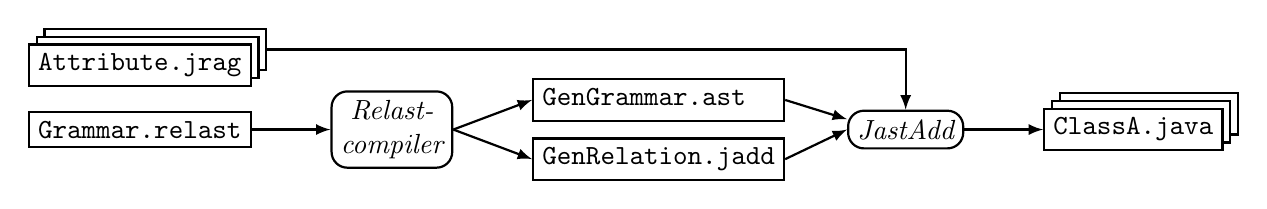
\begin{tikzpicture}
		\pgfdeclarelayer{bg}    % declare background layer
		\pgfsetlayers{bg,main}  % set the order of the layers (main is the standard layer)
		
		\tikzstyle{data} = [thick,minimum width=16,minimum height=10,draw,font=\ttfamily]
		\tikzstyle{process} = [thick,minimum width=16,minimum height=10,draw,font=\itshape,,rounded corners=2mm]
		\tikzstyle{myarrow} = [-latex,thick]
		
		% Nodes
		\node [data] (grammar) at (0,0) {Grammar.relast};
		\node [process, right=10mm of grammar, align=center] (relast) {Relast-\\compiler};
		\node [data, above right=-4mm and 10mm of relast] (genGrammar) {GenGrammar.ast\phantom{ja}};
		\node [data, below right=-4mm and 10mm of relast] (genRelation) {GenRelation.jadd};
		\node [process, right=50mm of relast] (jastadd) {JastAdd};
		
		% Attributes above grammar.relast
		\node [data, fill=white, above=3mm of grammar] (attr) {Attribute.jrag};
		\begin{pgfonlayer}{bg}    % select the background layer
		  \node [data, xshift=2mm,yshift=2mm] (attr2) at (attr) {\phantom{Attribute.jrag}};
		  \node [data, fill=white, xshift=1mm,yshift=1mm] at (attr) {\phantom{Attribute.jrag}};
		\end{pgfonlayer}
		\draw [myarrow] (attr2.east) -| (jastadd.north);
		
		\node [data, fill=white, right=10mm of jastadd] (java) {ClassA.java};
		\begin{pgfonlayer}{bg}    % select the background layer
		  \node [data, xshift=2mm,yshift=2mm] at (java) {\phantom{ClassA.java}};
		  \node [data, fill=white, xshift=1mm,yshift=1mm] at (java) {\phantom{ClassA.java}};
		\end{pgfonlayer}
		
		\draw [myarrow] (grammar.east) -- (relast.west);
		\draw [myarrow] (relast.east) -- (genGrammar.west);
		\draw [myarrow] (relast.east) -- (genRelation.west);
		\draw [myarrow] (genGrammar.east) -- (jastadd.170);
		\draw [myarrow] (genRelation.east) -- (jastadd.west);
		\draw [myarrow] (jastadd.east) -- (java.west);
	\end{tikzpicture}
\end{frame}

\begin{frame}
	\frametitle{Evaluation}
	Two aspects:
	\begin{enumerate}
		\item \textbf{Performance}
		\begin{itemize}
			\item Compare the three approaches with model- and graph-based solutions
		\end{itemize}
		\item \textbf{Conciseness}
		\begin{itemize}
			\item Measure complexity reduction
		\end{itemize}	
	\end{enumerate}
	
%	\begin{todolist}
%		\item Introduce the competition
%		\item All 6 queries
%		\item Mention the setting (which machine etc)
%		\item Part 1: LOC/shorter attributes (maybe diff?)
%		\item Part 2: show the diagrams from the paper.
%	\end{todolist}
\end{frame}

\begin{frame}
	\frametitle{The Train Benchmark}
	\includegraphics[width=.9\linewidth]{images/tb_process.pdf}\\
	\footnotesize{Benchmark process, from \todotext{cite train paper}}\normalsize
	
	\vspace{1\baselineskip}
	\begin{description}
		\item[\textbf{Read}] Load a model from file
		\item[\textbf{Check}] Perform a consistency check
		\item[\textbf{Transformation}] Fix some faults found during the preceding \emph{check}
		\item[\textbf{Recheck}] Repeat the check on the transformed model
	\end{description}
\end{frame}

\begin{frame}
	\frametitle{Example  Query: RouteSensor}
	\textbf{RouteSensor:}\\
	\includegraphics[width=.5\linewidth]{images/route_sensor_query.png}\\
	\footnotesize{RouteSensor pattern, from \todotext{cite train paper}}\normalsize
	
	\vspace{1\baselineskip}
	\begin{itemize}
		\item If a switch is \emph{monitored by} a sensor, the route that uses the switch must \emph{require} the sensor.
		\item If the above pattern is found, there is an error in the model.
	\end{itemize}
\end{frame}

\begin{frame}
	\frametitle{Example  Query: ConnectedSegments}
	\textbf{ConnectedSegments:}\\
	\includegraphics[width=.38\linewidth]{images/connected_segments_query.png}\\
	\footnotesize{ConnectedSegments pattern, from \todotext{cite train paper}}\normalsize
	
	\begin{itemize}
		\item A sensor must not monitor more than five segments in a row.
		\item If the above pattern is found, there is an error in the model.
	\end{itemize}
\end{frame}

\begin{frame}
	\frametitle{Performance}
	Comparing:
	\begin{itemize}
		\item Three RAG variants
		\begin{itemize}
			\item Name lookup
				\begin{tikzpicture}	
					% Namelookup incremental: rectangle
					\draw [fill=HKS07,draw=HKS07,line width=.5] rectangle (.2,.2);
					\draw [draw=HKS07,line width=1] (-.2,.1) -- (.4,.1);
				\end{tikzpicture}
			\item Intrinsic Reference Attributes
				\begin{tikzpicture}
					% Optimized incremental: circle
					\draw [fill=tudcyan,draw=tudcyan,line width=.5mm] circle (.1);
					\draw [draw=tudcyan,line width=1] (-.3,0) -- (.3,0);
				\end{tikzpicture}
			\item Grammar extension
					\begin{tikzpicture}
						% Namelookup incremental: unfilled rectangle
						\draw [fill=HKS65,draw=HKS65,line width=0] (.12,.24) -- (.24,0) -- (0,0);
						\draw [draw=HKS65,line width=1] (-.12,.1) -- (.36,.1);
					\end{tikzpicture}
		\end{itemize}
		\item A non-incremental graph database solution
		\begin{itemize}
			\item Tinkergraph \todotext{cite tinkergraph, maybe URL}
		\end{itemize}
		\item An incremental Java modeling solution
		\begin{itemize}
			\item Viatra \todotext{cite Viatra, maybe URL}
		\end{itemize}
	\end{itemize}
	
\end{frame}

% trim: left bottom right top
%% Read+Check
\begin{frame}
\frametitle{Read+Check: Route Sensor (Repair)}
	\absolutetikz{
		\node[anchor=north west] (pic) at (10mm,10mm) {\includegraphics[width=.5\linewidth,keepaspectratio,clip,trim=0cm 2.2cm 0cm 1.35cm]{images/repair-Read-and-Check-RouteSensor.pdf}};
    \node[anchor=north west,fill=white,xshift=-36mm,yshift=18mm] at (pic) {\rotatebox{90}{Execution time [ms]}};
    \node[anchor=north west,fill=white,align=center,xshift=-4mm,yshift=-20mm] at (pic) {Model size\\\#Elements};
    \node[anchor=north west] (legend) at (10mm,65mm) {\includegraphics[width=\linewidth,keepaspectratio]{images/diagram-legend}};
	}
\end{frame}

\begin{frame}
\frametitle{Read+Check: Connected Segments (Repair)}
	\absolutetikz{
		\node[anchor=north west] (pic) at (10mm,10mm) {\includegraphics[width=.5\linewidth,keepaspectratio,clip,trim=0cm 2.2cm 0cm 1.35cm]{images/repair-Read-and-Check-ConnectedSegments.pdf}};
    \node[anchor=north west,fill=white,xshift=-36mm,yshift=18mm] at (pic) {\rotatebox{90}{Execution time [ms]}};
    \node[anchor=north west,fill=white,align=center,xshift=-4mm,yshift=-20mm] at (pic) {Model size\\\#Elements};
    \node[anchor=north west] (legend) at (10mm,65mm) {\includegraphics[width=\linewidth,keepaspectratio]{images/diagram-legend}};
	}
\end{frame}

%% Transformation+Recheck (Inject)
\begin{frame}
\frametitle{Transformation+Recheck: Route Sensor (Inject)}
	\absolutetikz{
		\node[anchor=north west] (pic) at (10mm,10mm) {\includegraphics[width=.5\linewidth,keepaspectratio,clip,trim=0cm 2.2cm 0cm 1.35cm]{images/inject-Transformation-and-Recheck-RouteSensor.pdf}};
    \node[anchor=north west,fill=white,xshift=-36mm,yshift=18mm] at (pic) {\rotatebox{90}{Execution time [ms]}};
    \node[anchor=north west,fill=white,align=center,xshift=-4mm,yshift=-20mm] at (pic) {Model size\\\#Elements};
    \node[anchor=north west] (legend) at (10mm,65mm) {\includegraphics[width=\linewidth,keepaspectratio]{images/diagram-legend}};
	}
\end{frame}

\begin{frame}
\frametitle{Transformation+Recheck: Connected Segments (Inject)}
	\absolutetikz{
		\node[anchor=north west] (pic) at (10mm,10mm) {\includegraphics[width=.5\linewidth,keepaspectratio,clip,trim=0cm 2.2cm 0cm 1.35cm]{images/inject-Transformation-and-Recheck-ConnectedSegments.pdf}};
    \node[anchor=north west,fill=white,xshift=-36mm,yshift=18mm] at (pic) {\rotatebox{90}{Execution time [ms]}};
    \node[anchor=north west,fill=white,align=center,xshift=-4mm,yshift=-20mm] at (pic) {Model size\\\#Elements};
    \node[anchor=north west] (legend) at (10mm,65mm) {\includegraphics[width=\linewidth,keepaspectratio]{images/diagram-legend}};
	}
\end{frame}

%% Transformation+Recheck (Repair)
\begin{frame}
\frametitle{Transformation+Recheck: Route Sensor (Repair)}
	\absolutetikz{
		\node[anchor=north west] (pic) at (10mm,10mm) {\includegraphics[width=.5\linewidth,keepaspectratio,clip,trim=0cm 2.2cm 0cm 1.35cm]{images/repair-Transformation-and-Recheck-RouteSensor.pdf}};
    \node[anchor=north west,fill=white,xshift=-36mm,yshift=18mm] at (pic) {\rotatebox{90}{Execution time [ms]}};
    \node[anchor=north west,fill=white,align=center,xshift=-4mm,yshift=-20mm] at (pic) {Model size\\\#Elements};
    \node[anchor=north west] (legend) at (10mm,65mm) {\includegraphics[width=\linewidth,keepaspectratio]{images/diagram-legend}};
	}
\end{frame}

\begin{frame}
\frametitle{Transformation+Recheck: Connected Segments (Repair)}
	\absolutetikz{
		\node[anchor=north west] (pic) at (10mm,10mm) {\includegraphics[width=.5\linewidth,keepaspectratio,clip,trim=0cm 2.2cm 0cm 1.35cm]{images/repair-Transformation-and-Recheck-ConnectedSegments.pdf}};
    \node[anchor=north west,fill=white,xshift=-36mm,yshift=18mm] at (pic) {\rotatebox{90}{Execution time [ms]}};
    \node[anchor=north west,fill=white,align=center,xshift=-4mm,yshift=-20mm] at (pic) {Model size\\\#Elements};
    \node[anchor=north west] (legend) at (10mm,65mm) {\includegraphics[width=\linewidth,keepaspectratio]{images/diagram-legend}};
	}
\end{frame}


\begin{frame}
	\frametitle{Results}
	\begin{itemize}
		\item Performs on par with state-of-the-art incremental model tools
		\item Faster for some queries
		\item Opens possibility for RAGs on Models
	\end{itemize}
\end{frame}

\end{document}
